\documentclass[11pt]{article}
\usepackage[textwidth=18.0cm, textheight=23.0cm, top=2.0cm]{geometry}
\usepackage{pst-all}
\usepackage{amssymb}
\usepackage{tikz}
\usepackage{underscore}\begin{document}
\pagestyle{empty}


ClassName: \underline{\textbf{Class_10.2bp-14}}
\par
BinSize: \underline{\textbf{100 × 100}}
\par
ReduceSize: \underline{\textbf{100 × 100}}
\par
TypeNum: \underline{\textbf{39}}
\par
Num: \underline{\textbf{40}}
\par
OutS: \underline{\textbf{60000}}
\par
InS: \underline{\textbf{50594}}
\par
Rate: \underline{\textbf{0.843}}
\par
UB: \underline{\textbf{6}}
\par
LB0: \underline{\textbf{6}}
\par
LB: \underline{\textbf{6}}
\par
LBWithCut: \underline{\textbf{6}}
\par
NodeCut: \underline{\textbf{0}}
\par
ExtendedNodeCnt: \underline{\textbf{1}}
\par
GenNodeCnt: \underline{\textbf{1}}
\par
PrimalNode: \underline{\textbf{0}}
\par
ColumnCount: \underline{\textbf{6}}
\par
TotalCutCount: \underline{\textbf{0}}
\par
RootCutCount: \underline{\textbf{0}}
\par
LPSolverCnt: \underline{\textbf{1}}
\par
PricingSolverCnt: \underline{\textbf{0}}
\par
BranchAndBoundNum: \underline{\textbf{1}}
\par
isOpt: \underline{\textbf{true}}
\par
TimeOnInitSolution: \underline{\textbf{600.000 s}}
\par
TimeOnPrimal: \underline{\textbf{0.000 s}}
\par
TimeOnPricing: \underline{\textbf{0.000 s}}
\par
TimeOnRmp: \underline{\textbf{0.062 s}}
\par
TotalTime: \underline{\textbf{600.312 s}}
\par
\newpage


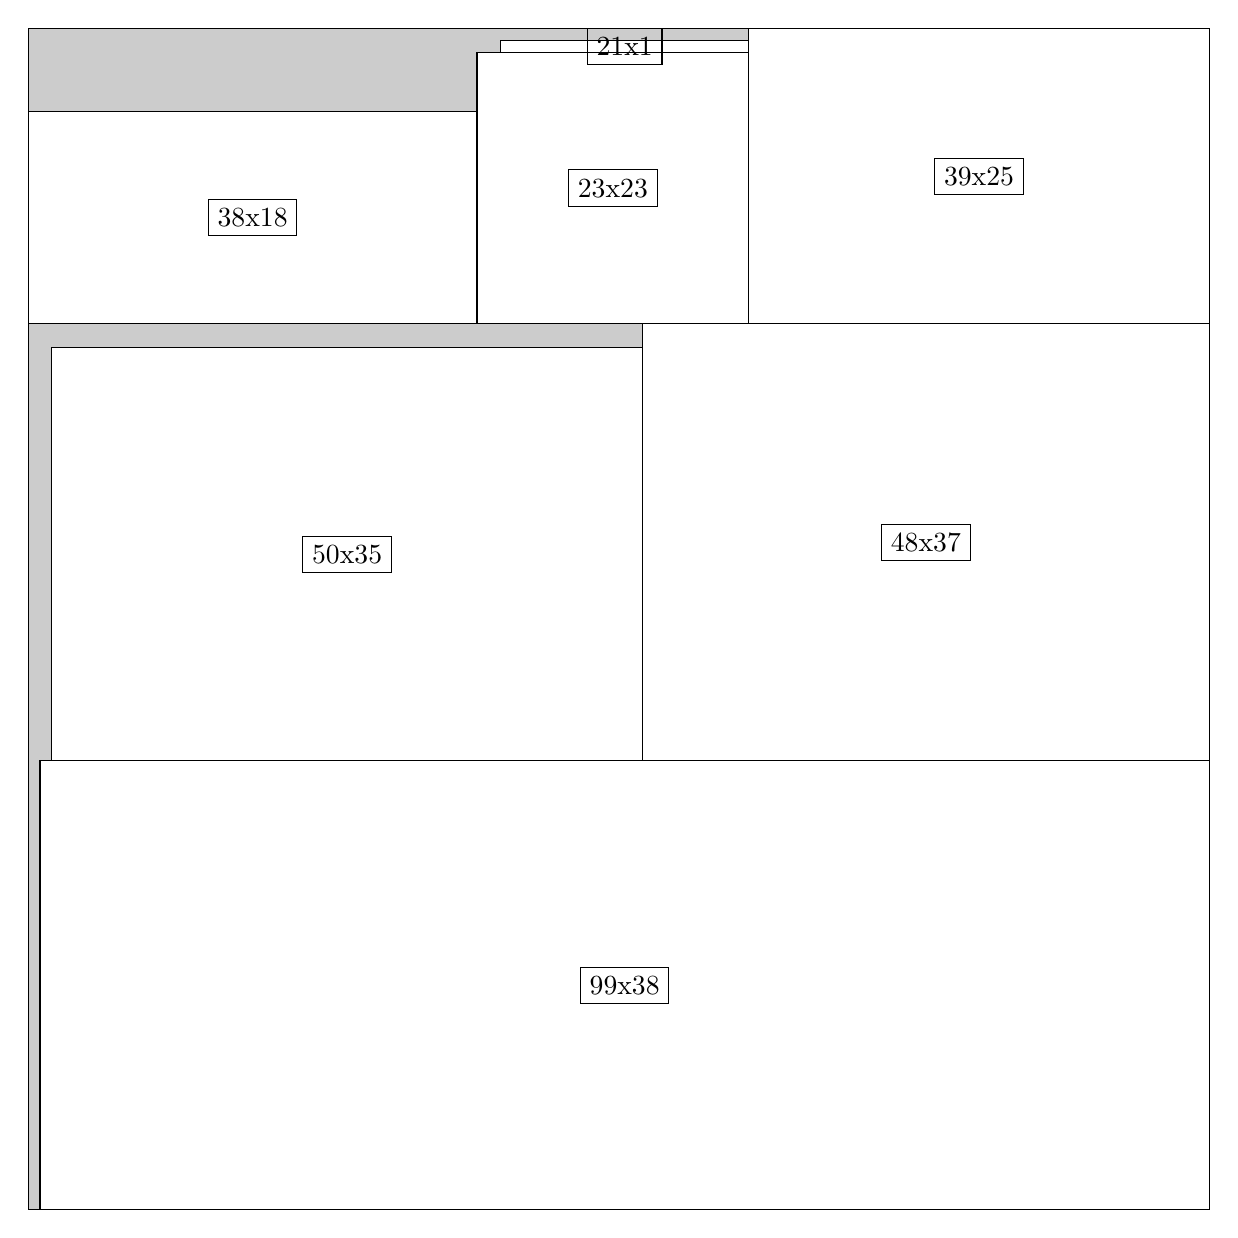
\begin{tikzpicture}[shorten >=1pt,scale=1.0,every node/.style={scale=1.0},->]
\tikzstyle{vertex}=[circle,fill=black!25,minimum size=14pt,inner sep=0pt]
\filldraw[fill=gray!40!white, draw=black] (0,0) rectangle (15.0,15.0);
\foreach \name/\x/\y/\w/\h in {99x38/0.15/0.0/14.85/5.7,48x37/7.8/5.7/7.199999999999999/5.55,50x35/0.3/5.7/7.5/5.25,39x25/9.15/11.25/5.85/3.75,23x23/5.7/11.25/3.4499999999999997/3.4499999999999997,21x1/6.0/14.7/3.15/0.15,38x18/0.0/11.25/5.7/2.6999999999999997}
\filldraw[fill=white!40!white, draw=black] (\x,\y) rectangle node[draw] (\name) {\name} ++(\w,\h);
\end{tikzpicture}


w =99 , h =38 , x =1 , y =0 , v =3762
\par
w =48 , h =37 , x =52 , y =38 , v =1776
\par
w =50 , h =35 , x =2 , y =38 , v =1750
\par
w =39 , h =25 , x =61 , y =75 , v =975
\par
w =23 , h =23 , x =38 , y =75 , v =529
\par
w =21 , h =1 , x =40 , y =98 , v =21
\par
w =38 , h =18 , x =0 , y =75 , v =684
\par
\newpage


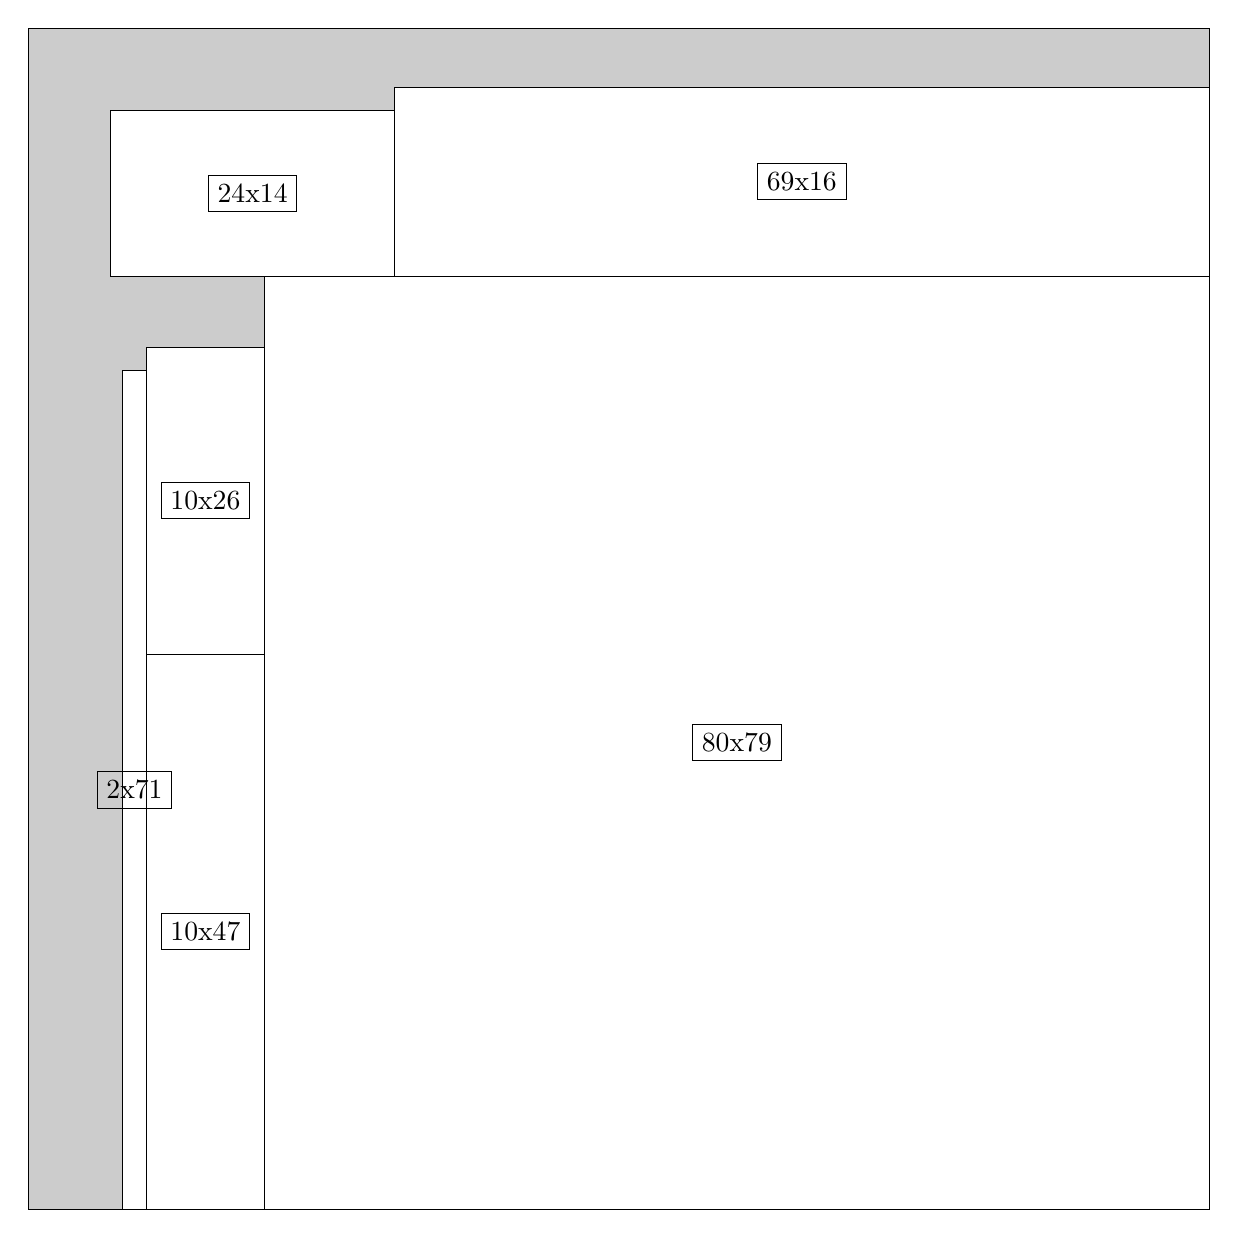
\begin{tikzpicture}[shorten >=1pt,scale=1.0,every node/.style={scale=1.0},->]
\tikzstyle{vertex}=[circle,fill=black!25,minimum size=14pt,inner sep=0pt]
\filldraw[fill=gray!40!white, draw=black] (0,0) rectangle (15.0,15.0);
\foreach \name/\x/\y/\w/\h in {80x79/3.0/0.0/12.0/11.85,10x47/1.5/0.0/1.5/7.05,10x26/1.5/7.05/1.5/3.9,2x71/1.2/0.0/0.3/10.65,69x16/4.6499999999999995/11.85/10.35/2.4,24x14/1.05/11.85/3.5999999999999996/2.1}
\filldraw[fill=white!40!white, draw=black] (\x,\y) rectangle node[draw] (\name) {\name} ++(\w,\h);
\end{tikzpicture}


w =80 , h =79 , x =20 , y =0 , v =6320
\par
w =10 , h =47 , x =10 , y =0 , v =470
\par
w =10 , h =26 , x =10 , y =47 , v =260
\par
w =2 , h =71 , x =8 , y =0 , v =142
\par
w =69 , h =16 , x =31 , y =79 , v =1104
\par
w =24 , h =14 , x =7 , y =79 , v =336
\par
\newpage


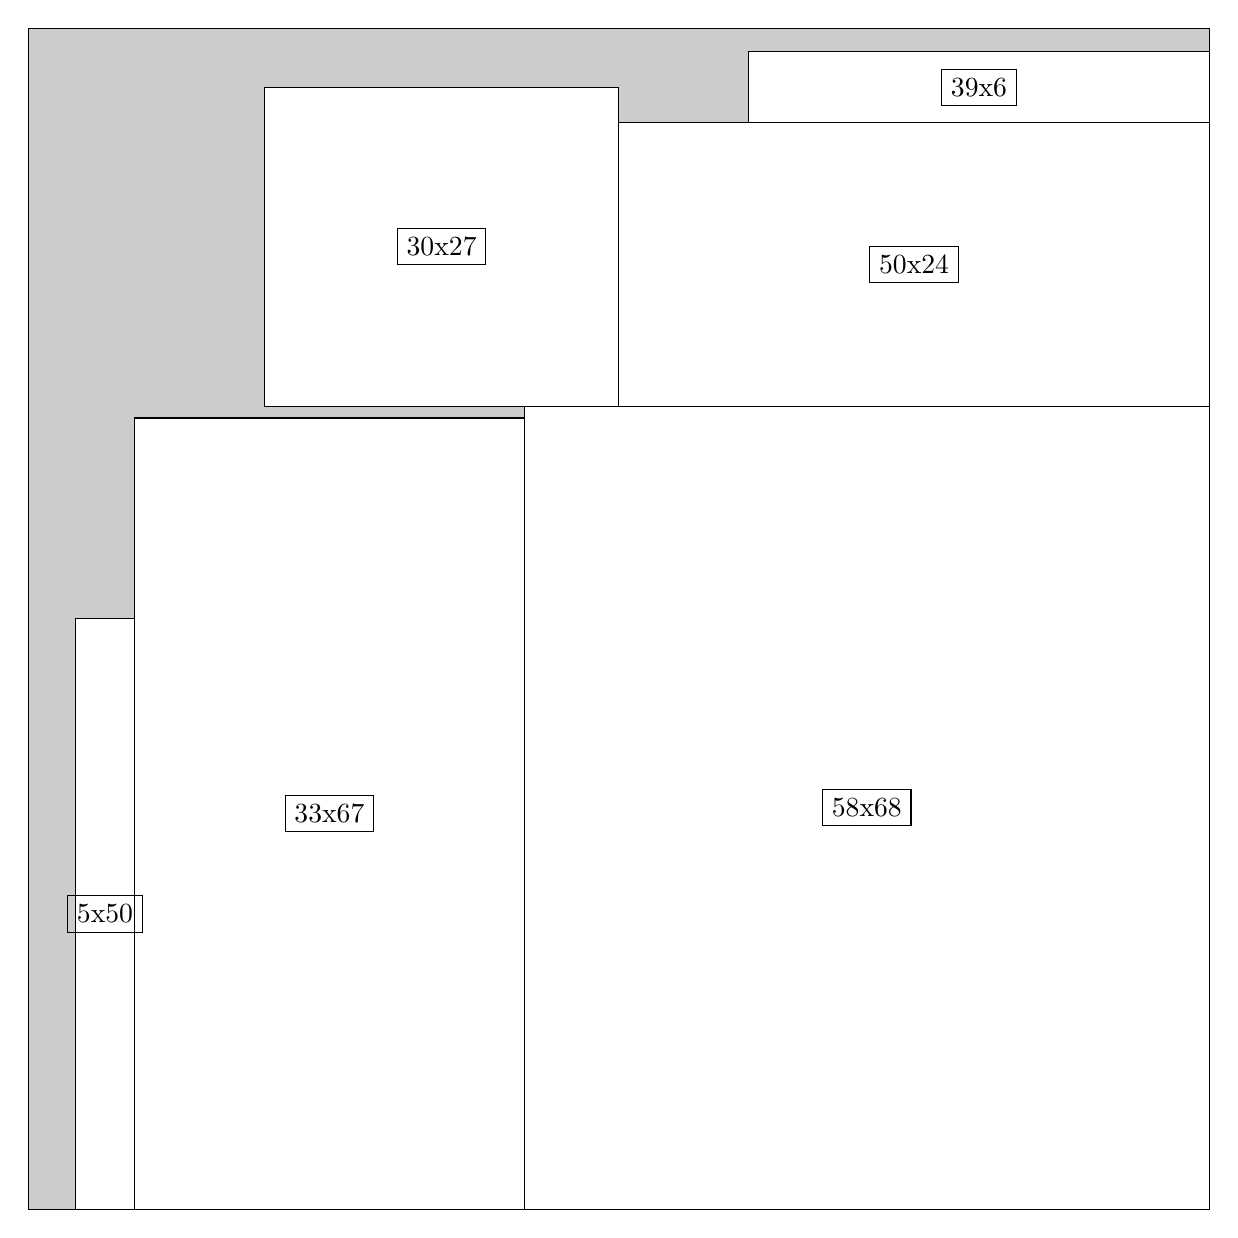
\begin{tikzpicture}[shorten >=1pt,scale=1.0,every node/.style={scale=1.0},->]
\tikzstyle{vertex}=[circle,fill=black!25,minimum size=14pt,inner sep=0pt]
\filldraw[fill=gray!40!white, draw=black] (0,0) rectangle (15.0,15.0);
\foreach \name/\x/\y/\w/\h in {58x68/6.3/0.0/8.7/10.2,33x67/1.3499999999999999/0.0/4.95/10.049999999999999,5x50/0.6/0.0/0.75/7.5,50x24/7.5/10.2/7.5/3.5999999999999996,39x6/9.15/13.799999999999999/5.85/0.8999999999999999,30x27/3.0/10.2/4.5/4.05}
\filldraw[fill=white!40!white, draw=black] (\x,\y) rectangle node[draw] (\name) {\name} ++(\w,\h);
\end{tikzpicture}


w =58 , h =68 , x =42 , y =0 , v =3944
\par
w =33 , h =67 , x =9 , y =0 , v =2211
\par
w =5 , h =50 , x =4 , y =0 , v =250
\par
w =50 , h =24 , x =50 , y =68 , v =1200
\par
w =39 , h =6 , x =61 , y =92 , v =234
\par
w =30 , h =27 , x =20 , y =68 , v =810
\par
\newpage


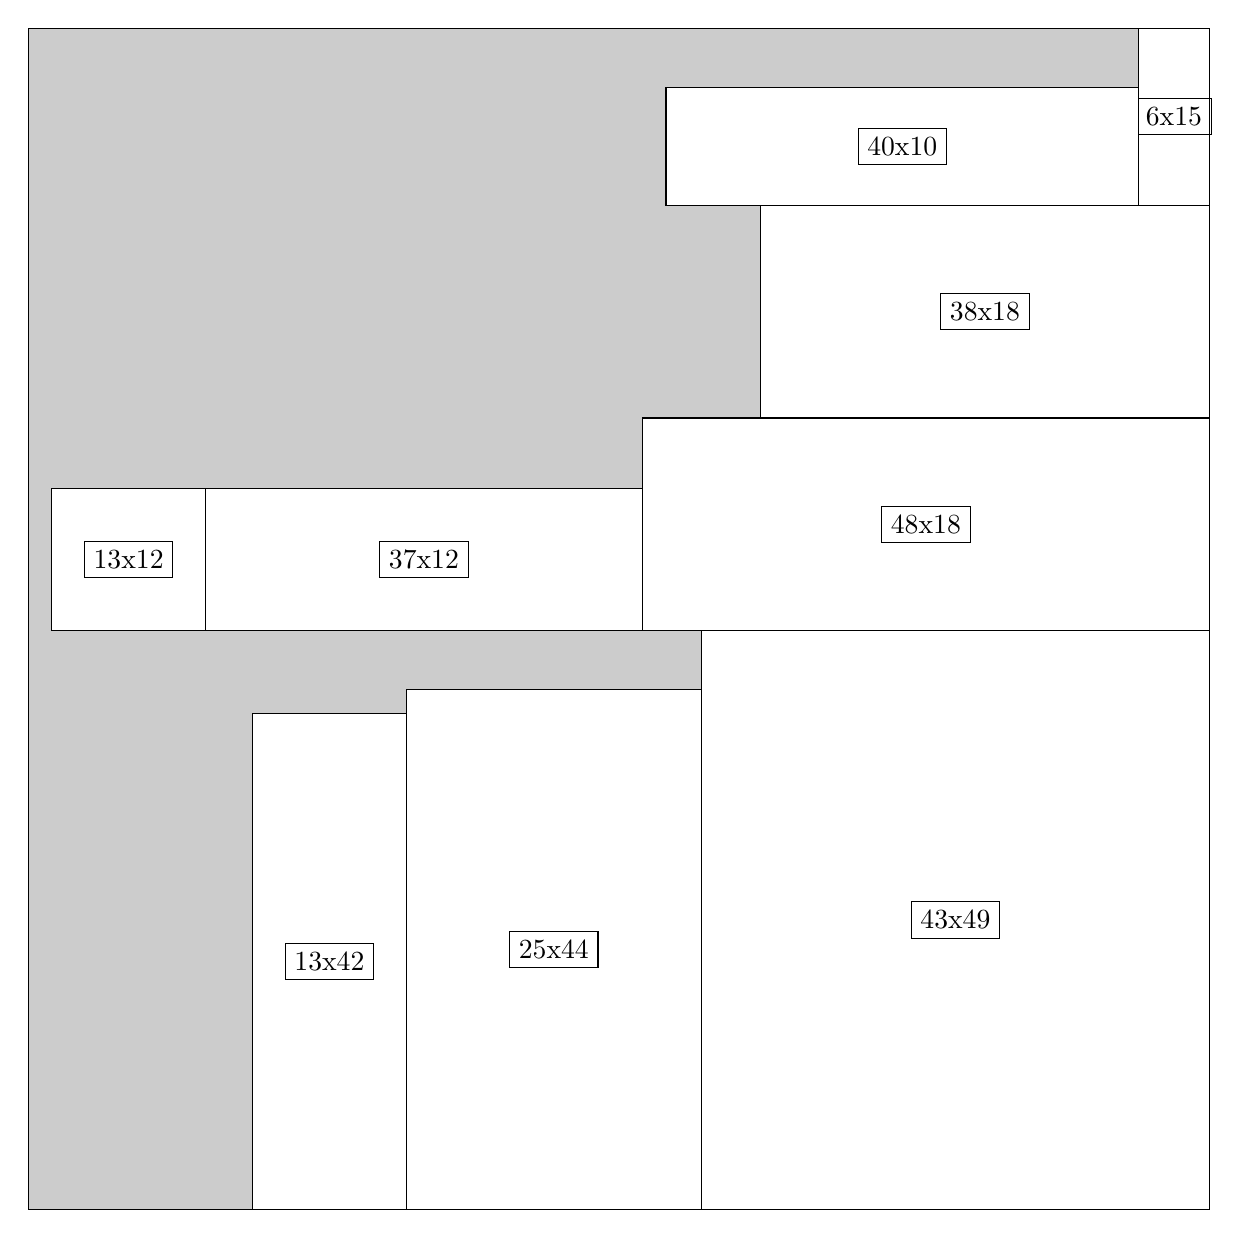
\begin{tikzpicture}[shorten >=1pt,scale=1.0,every node/.style={scale=1.0},->]
\tikzstyle{vertex}=[circle,fill=black!25,minimum size=14pt,inner sep=0pt]
\filldraw[fill=gray!40!white, draw=black] (0,0) rectangle (15.0,15.0);
\foreach \name/\x/\y/\w/\h in {43x49/8.549999999999999/0.0/6.45/7.35,25x44/4.8/0.0/3.75/6.6,13x42/2.85/0.0/1.95/6.3,48x18/7.8/7.35/7.199999999999999/2.6999999999999997,38x18/9.299999999999999/10.049999999999999/5.7/2.6999999999999997,6x15/14.1/12.75/0.8999999999999999/2.25,40x10/8.1/12.75/6.0/1.5,37x12/2.25/7.35/5.55/1.7999999999999998,13x12/0.3/7.35/1.95/1.7999999999999998}
\filldraw[fill=white!40!white, draw=black] (\x,\y) rectangle node[draw] (\name) {\name} ++(\w,\h);
\end{tikzpicture}


w =43 , h =49 , x =57 , y =0 , v =2107
\par
w =25 , h =44 , x =32 , y =0 , v =1100
\par
w =13 , h =42 , x =19 , y =0 , v =546
\par
w =48 , h =18 , x =52 , y =49 , v =864
\par
w =38 , h =18 , x =62 , y =67 , v =684
\par
w =6 , h =15 , x =94 , y =85 , v =90
\par
w =40 , h =10 , x =54 , y =85 , v =400
\par
w =37 , h =12 , x =15 , y =49 , v =444
\par
w =13 , h =12 , x =2 , y =49 , v =156
\par
\newpage


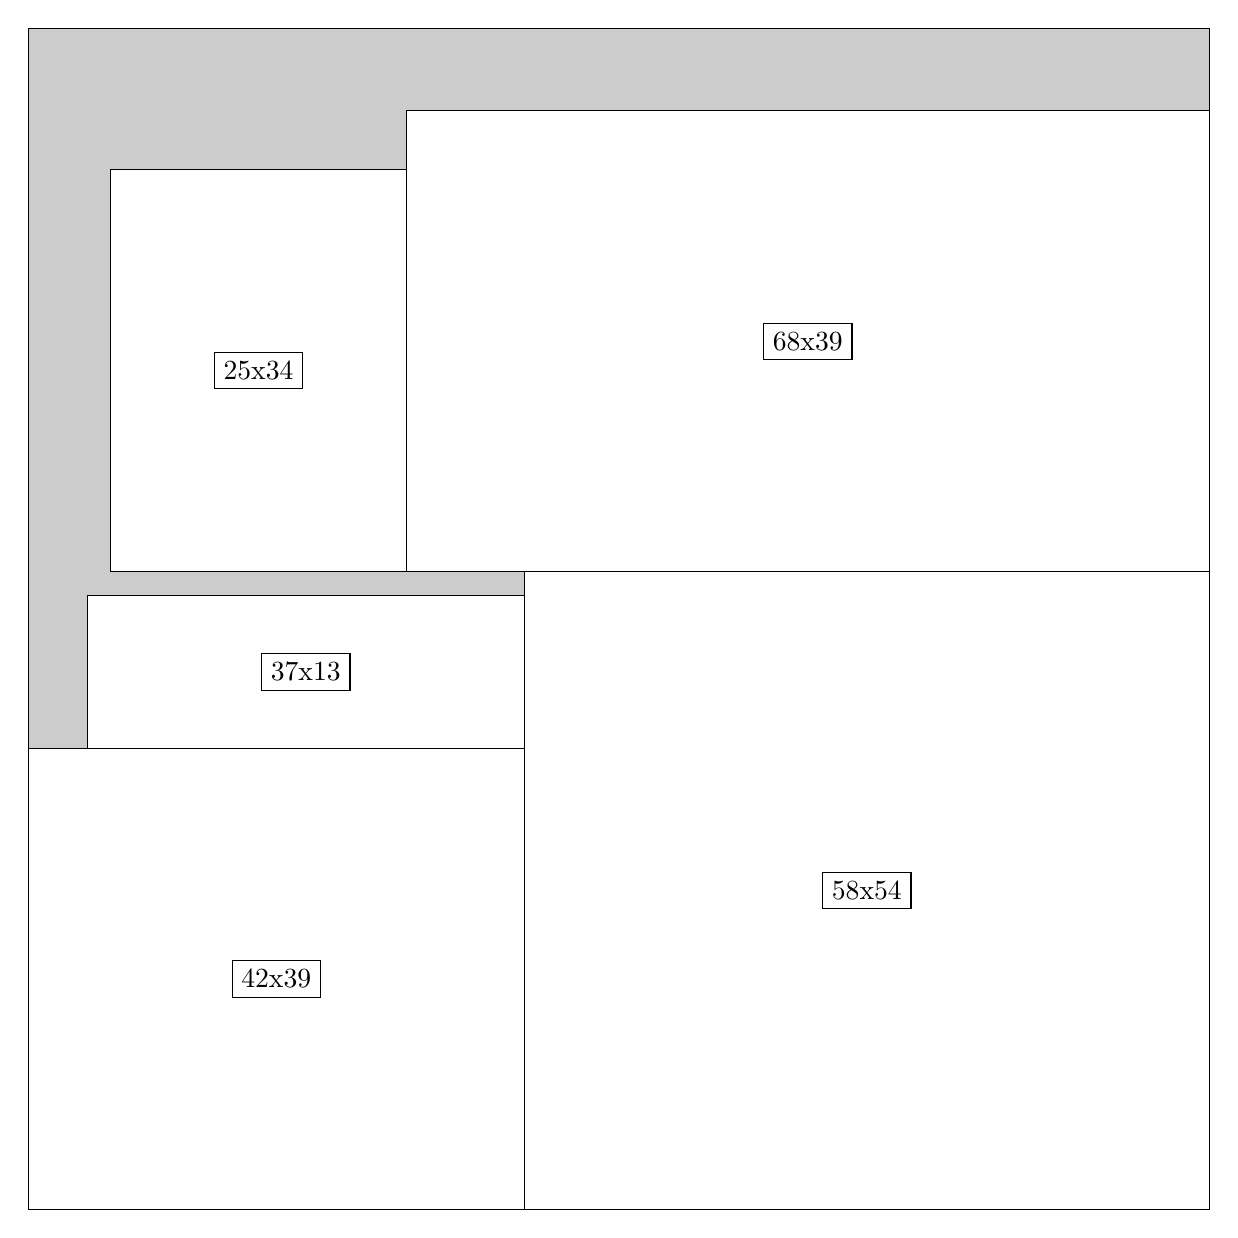
\begin{tikzpicture}[shorten >=1pt,scale=1.0,every node/.style={scale=1.0},->]
\tikzstyle{vertex}=[circle,fill=black!25,minimum size=14pt,inner sep=0pt]
\filldraw[fill=gray!40!white, draw=black] (0,0) rectangle (15.0,15.0);
\foreach \name/\x/\y/\w/\h in {58x54/6.3/0.0/8.7/8.1,42x39/0.0/0.0/6.3/5.85,37x13/0.75/5.85/5.55/1.95,68x39/4.8/8.1/10.2/5.85,25x34/1.05/8.1/3.75/5.1}
\filldraw[fill=white!40!white, draw=black] (\x,\y) rectangle node[draw] (\name) {\name} ++(\w,\h);
\end{tikzpicture}


w =58 , h =54 , x =42 , y =0 , v =3132
\par
w =42 , h =39 , x =0 , y =0 , v =1638
\par
w =37 , h =13 , x =5 , y =39 , v =481
\par
w =68 , h =39 , x =32 , y =54 , v =2652
\par
w =25 , h =34 , x =7 , y =54 , v =850
\par
\newpage


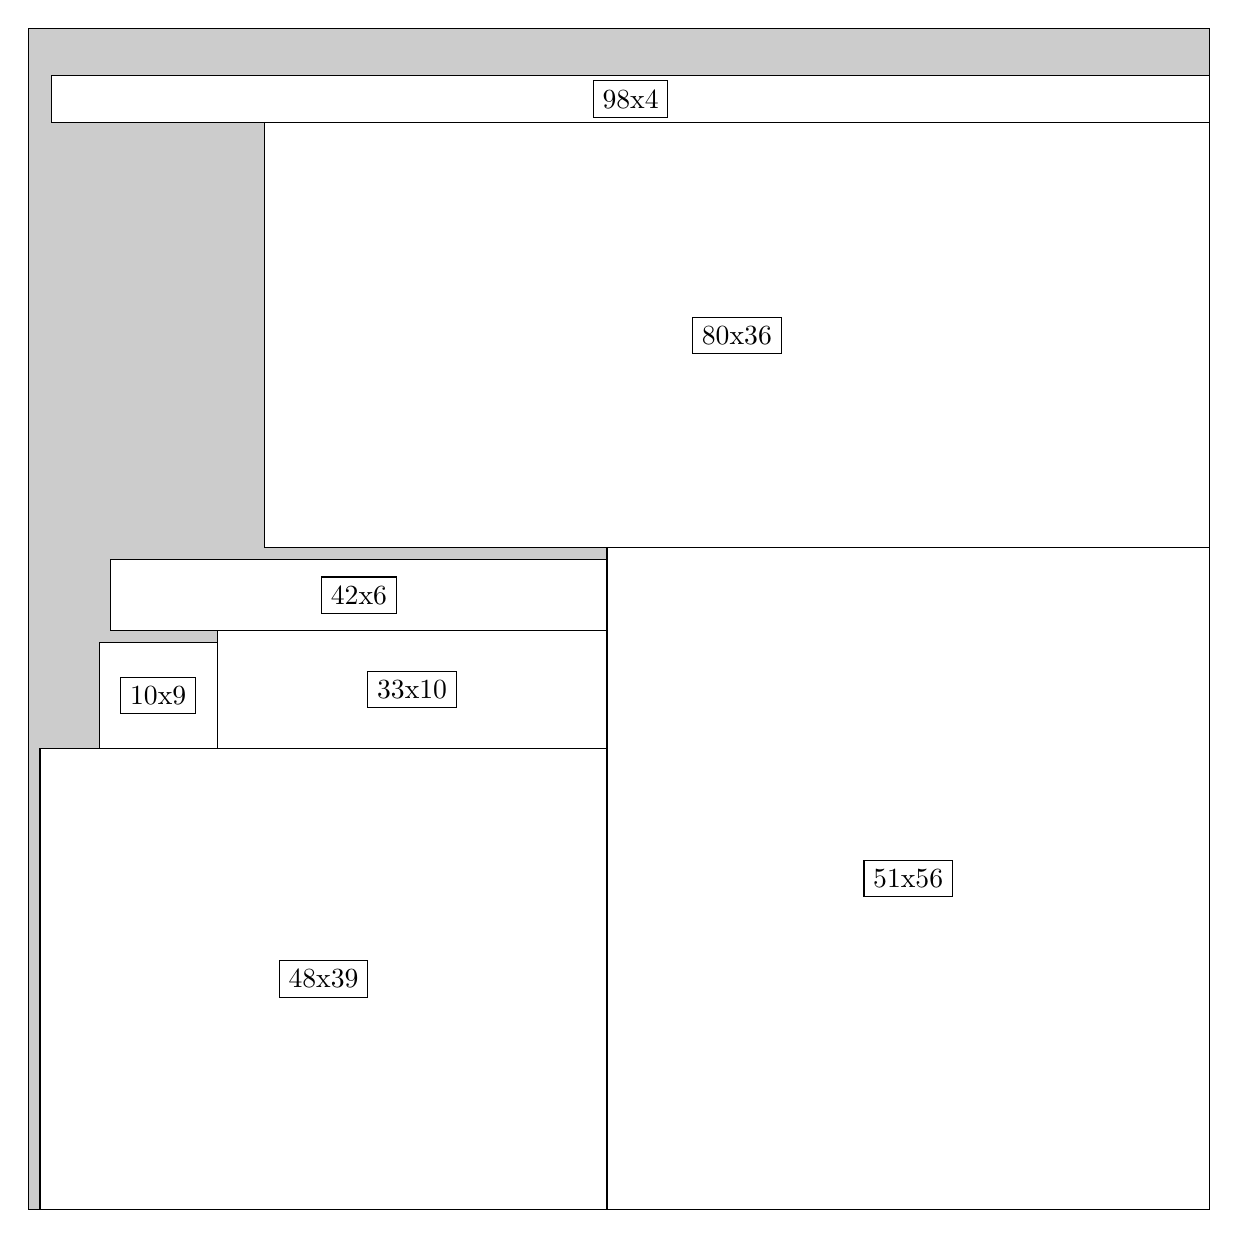
\begin{tikzpicture}[shorten >=1pt,scale=1.0,every node/.style={scale=1.0},->]
\tikzstyle{vertex}=[circle,fill=black!25,minimum size=14pt,inner sep=0pt]
\filldraw[fill=gray!40!white, draw=black] (0,0) rectangle (15.0,15.0);
\foreach \name/\x/\y/\w/\h in {51x56/7.35/0.0/7.6499999999999995/8.4,48x39/0.15/0.0/7.199999999999999/5.85,33x10/2.4/5.85/4.95/1.5,10x9/0.8999999999999999/5.85/1.5/1.3499999999999999,42x6/1.05/7.35/6.3/0.8999999999999999,80x36/3.0/8.4/12.0/5.3999999999999995,98x4/0.3/13.799999999999999/14.7/0.6}
\filldraw[fill=white!40!white, draw=black] (\x,\y) rectangle node[draw] (\name) {\name} ++(\w,\h);
\end{tikzpicture}


w =51 , h =56 , x =49 , y =0 , v =2856
\par
w =48 , h =39 , x =1 , y =0 , v =1872
\par
w =33 , h =10 , x =16 , y =39 , v =330
\par
w =10 , h =9 , x =6 , y =39 , v =90
\par
w =42 , h =6 , x =7 , y =49 , v =252
\par
w =80 , h =36 , x =20 , y =56 , v =2880
\par
w =98 , h =4 , x =2 , y =92 , v =392
\par
\newpage


\end{document}